%%%% Preamble %%%%
\documentclass[a4paper, oneside, 10pt]{article}

% wider text, smaller margins
\usepackage{a4wide}

% font choice
\usepackage[utf8]{inputenc}
% \usepackage{kpfonts}
\usepackage[T1]{fontenc}
% \usepackage{newtxtext,newtxmath}

% for coloring
\usepackage[dvipsnames]{xcolor}

% for index list
\usepackage{makeidx}
\makeindex

% for better lists
\usepackage{enumitem}

% for images
\usepackage{graphicx}
\graphicspath{{./Pics/}}

% for hyperrefs
\usepackage{hyperref}

% for declaring math operators
\usepackage{amsthm}

% wrap text around figures
\usepackage{wrapfig}

% chagne format of section titles
\usepackage{titlesec}

% \titleformat*{\section}{\LARGE\bfseries}
% \titleformat*{\subsection}{\Large\bfseries}
% \titleformat*{\subsubsection}{\large\bfseries}
\titleformat*{\paragraph}{\bfseries\itshape}
% \titleformat*{\subparagraph}{\large\bfseries}

% nice text boxes
\usepackage{tcolorbox}
\newtcbox{\note}{on line, boxrule=0pt, boxsep=0pt, arc=0pt, outer arc=0pt, left=1pt, right=1pt, top=2pt, bottom=2pt, fontupper=\itshape}
% \newtcolorbox{notebox}{boxrule=0pt}
\newtcolorbox{notebox}[1][colback=black!5]{boxrule=0pt, #1}

% biblatex seetings for better referencing
\usepackage[backend=biber,
            citestyle=authoryear,
            bibstyle=numeric,
            block=space,
            backref=true,
            date=year,
            maxcitenames=2,
            mincitenames=1,
            url=false,
            doi=false,
            isbn=false,
            eprint=false]{biblatex}
\addbibresource{refs.bib}


%%% theorem environments
\theoremstyle{plain}
\newtheoremstyle{mytheoremstyle} % name
    {\topsep}{\topsep}{}{}%
    {\bfseries}% Theorem head font
    {}{.5em}%
    {\thmname{#1}\thmnumber{ #2}\thmnote{ (#3)}}  % Theorem head spec (can be left empty, meaning ‘normal’)
\theoremstyle{mytheoremstyle}
\newtheorem{theorem}{Theorem}[section]

\theoremstyle{definition}
\newtheoremstyle{mydefstyle} % name
    {\topsep}{\partopsep}{}{}%
    {\bfseries}% Theorem head font
    {}{.5em}%
    {\thmname{#1}\thmnumber{ #2}\thmnote{ (#3)}}  % Theorem head spec (can be left empty, meaning ‘normal’)
\theoremstyle{mydefstyle}
\newtheorem{definition}{Definition}[section]

%%%%% NEW MATH DEFINITIONS %%%%%

\usepackage{amsmath,amsfonts,bm}

% Mark sections of captions for referring to divisions of figures
\newcommand{\figleft}{{\em (Left)}}
\newcommand{\figcenter}{{\em (Center)}}
\newcommand{\figright}{{\em (Right)}}
\newcommand{\figtop}{{\em (Top)}}
\newcommand{\figbottom}{{\em (Bottom)}}
\newcommand{\captiona}{{\em (a)}}
\newcommand{\captionb}{{\em (b)}}
\newcommand{\captionc}{{\em (c)}}
\newcommand{\captiond}{{\em (d)}}

% Highlight a newly defined term
\newcommand{\iterm}[1]{{\emph{#1}\index{#1}}}


% Figure reference, lower-case.
\def\figref#1{figure~\ref{#1}}
% Figure reference, capital. For start of sentence
\def\Figref#1{Figure~\ref{#1}}
\def\twofigref#1#2{figures \ref{#1} and \ref{#2}}
\def\quadfigref#1#2#3#4{figures \ref{#1}, \ref{#2}, \ref{#3} and \ref{#4}}
% Section reference, lower-case.
\def\secref#1{section~\ref{#1}}
% Section reference, capital.
\def\Secref#1{Section~\ref{#1}}
% Reference to two sections.
\def\twosecrefs#1#2{sections \ref{#1} and \ref{#2}}
% Reference to three sections.
\def\secrefs#1#2#3{sections \ref{#1}, \ref{#2} and \ref{#3}}
% % Reference to an equation, lower-case.
% \def\eqref#1{equation~\ref{#1}}
% % Reference to an equation, upper case
% \def\Eqref#1{Equation~\ref{#1}}
% % A raw reference to an equation---avoid using if possible
% \def\plaineqref#1{\ref{#1}}
% Reference to a chapter, lower-case.
\def\chapref#1{chapter~\ref{#1}}
% Reference to an equation, upper case.
\def\Chapref#1{Chapter~\ref{#1}}
% Reference to a range of chapters
\def\rangechapref#1#2{chapters\ref{#1}--\ref{#2}}
% Reference to an algorithm, lower-case.
\def\algref#1{algorithm~\ref{#1}}
% Reference to an algorithm, upper case.
\def\Algref#1{Algorithm~\ref{#1}}
\def\twoalgref#1#2{algorithms \ref{#1} and \ref{#2}}
\def\Twoalgref#1#2{Algorithms \ref{#1} and \ref{#2}}
% Reference to a part, lower case
\def\partref#1{part~\ref{#1}}
% Reference to a part, upper case
\def\Partref#1{Part~\ref{#1}}
\def\twopartref#1#2{parts \ref{#1} and \ref{#2}}

\def\ceil#1{\lceil #1 \rceil}
\def\floor#1{\lfloor #1 \rfloor}
\def\1{\bm{1}}
\newcommand{\train}{\mathcal{D}}
\newcommand{\valid}{\mathcal{D_{\mathrm{valid}}}}
\newcommand{\test}{\mathcal{D_{\mathrm{test}}}}

\def\eps{{\epsilon}}


% Random variables
\def\reta{{\textnormal{$\eta$}}}
\def\ra{{\textnormal{a}}}
\def\rb{{\textnormal{b}}}
\def\rc{{\textnormal{c}}}
\def\rd{{\textnormal{d}}}
\def\re{{\textnormal{e}}}
\def\rf{{\textnormal{f}}}
\def\rg{{\textnormal{g}}}
\def\rh{{\textnormal{h}}}
\def\ri{{\textnormal{i}}}
\def\rj{{\textnormal{j}}}
\def\rk{{\textnormal{k}}}
\def\rl{{\textnormal{l}}}
% rm is already a command, just don't name any random variables m
\def\rn{{\textnormal{n}}}
\def\ro{{\textnormal{o}}}
\def\rp{{\textnormal{p}}}
\def\rq{{\textnormal{q}}}
\def\rr{{\textnormal{r}}}
\def\rs{{\textnormal{s}}}
\def\rt{{\textnormal{t}}}
\def\ru{{\textnormal{u}}}
\def\rv{{\textnormal{v}}}
\def\rw{{\textnormal{w}}}
\def\rx{{\textnormal{x}}}
\def\ry{{\textnormal{y}}}
\def\rz{{\textnormal{z}}}

% Random vectors
\def\rvepsilon{{\mathbf{\epsilon}}}
\def\rvtheta{{\mathbf{\theta}}}
\def\rva{{\mathbf{a}}}
\def\rvb{{\mathbf{b}}}
\def\rvc{{\mathbf{c}}}
\def\rvd{{\mathbf{d}}}
\def\rve{{\mathbf{e}}}
\def\rvf{{\mathbf{f}}}
\def\rvg{{\mathbf{g}}}
\def\rvh{{\mathbf{h}}}
\def\rvu{{\mathbf{i}}}
\def\rvj{{\mathbf{j}}}
\def\rvk{{\mathbf{k}}}
\def\rvl{{\mathbf{l}}}
\def\rvm{{\mathbf{m}}}
\def\rvn{{\mathbf{n}}}
\def\rvo{{\mathbf{o}}}
\def\rvp{{\mathbf{p}}}
\def\rvq{{\mathbf{q}}}
\def\rvr{{\mathbf{r}}}
\def\rvs{{\mathbf{s}}}
\def\rvt{{\mathbf{t}}}
\def\rvu{{\mathbf{u}}}
\def\rvv{{\mathbf{v}}}
\def\rvw{{\mathbf{w}}}
\def\rvx{{\mathbf{x}}}
\def\rvy{{\mathbf{y}}}
\def\rvz{{\mathbf{z}}}

% Elements of random vectors
\def\erva{{\textnormal{a}}}
\def\ervb{{\textnormal{b}}}
\def\ervc{{\textnormal{c}}}
\def\ervd{{\textnormal{d}}}
\def\erve{{\textnormal{e}}}
\def\ervf{{\textnormal{f}}}
\def\ervg{{\textnormal{g}}}
\def\ervh{{\textnormal{h}}}
\def\ervi{{\textnormal{i}}}
\def\ervj{{\textnormal{j}}}
\def\ervk{{\textnormal{k}}}
\def\ervl{{\textnormal{l}}}
\def\ervm{{\textnormal{m}}}
\def\ervn{{\textnormal{n}}}
\def\ervo{{\textnormal{o}}}
\def\ervp{{\textnormal{p}}}
\def\ervq{{\textnormal{q}}}
\def\ervr{{\textnormal{r}}}
\def\ervs{{\textnormal{s}}}
\def\ervt{{\textnormal{t}}}
\def\ervu{{\textnormal{u}}}
\def\ervv{{\textnormal{v}}}
\def\ervw{{\textnormal{w}}}
\def\ervx{{\textnormal{x}}}
\def\ervy{{\textnormal{y}}}
\def\ervz{{\textnormal{z}}}

% Random matrices
\def\rmA{{\mathbf{A}}}
\def\rmB{{\mathbf{B}}}
\def\rmC{{\mathbf{C}}}
\def\rmD{{\mathbf{D}}}
\def\rmE{{\mathbf{E}}}
\def\rmF{{\mathbf{F}}}
\def\rmG{{\mathbf{G}}}
\def\rmH{{\mathbf{H}}}
\def\rmI{{\mathbf{I}}}
\def\rmJ{{\mathbf{J}}}
\def\rmK{{\mathbf{K}}}
\def\rmL{{\mathbf{L}}}
\def\rmM{{\mathbf{M}}}
\def\rmN{{\mathbf{N}}}
\def\rmO{{\mathbf{O}}}
\def\rmP{{\mathbf{P}}}
\def\rmQ{{\mathbf{Q}}}
\def\rmR{{\mathbf{R}}}
\def\rmS{{\mathbf{S}}}
\def\rmT{{\mathbf{T}}}
\def\rmU{{\mathbf{U}}}
\def\rmV{{\mathbf{V}}}
\def\rmW{{\mathbf{W}}}
\def\rmX{{\mathbf{X}}}
\def\rmY{{\mathbf{Y}}}
\def\rmZ{{\mathbf{Z}}}

% Elements of random matrices
\def\ermA{{\textnormal{A}}}
\def\ermB{{\textnormal{B}}}
\def\ermC{{\textnormal{C}}}
\def\ermD{{\textnormal{D}}}
\def\ermE{{\textnormal{E}}}
\def\ermF{{\textnormal{F}}}
\def\ermG{{\textnormal{G}}}
\def\ermH{{\textnormal{H}}}
\def\ermI{{\textnormal{I}}}
\def\ermJ{{\textnormal{J}}}
\def\ermK{{\textnormal{K}}}
\def\ermL{{\textnormal{L}}}
\def\ermM{{\textnormal{M}}}
\def\ermN{{\textnormal{N}}}
\def\ermO{{\textnormal{O}}}
\def\ermP{{\textnormal{P}}}
\def\ermQ{{\textnormal{Q}}}
\def\ermR{{\textnormal{R}}}
\def\ermS{{\textnormal{S}}}
\def\ermT{{\textnormal{T}}}
\def\ermU{{\textnormal{U}}}
\def\ermV{{\textnormal{V}}}
\def\ermW{{\textnormal{W}}}
\def\ermX{{\textnormal{X}}}
\def\ermY{{\textnormal{Y}}}
\def\ermZ{{\textnormal{Z}}}

% Vectors
\def\vzero{{\bm{0}}}
\def\vone{{\bm{1}}}
\def\vmu{{\bm{\mu}}}
\def\vtheta{{\bm{\theta}}}
\def\va{{\bm{a}}}
\def\vb{{\bm{b}}}
\def\vc{{\bm{c}}}
\def\vd{{\bm{d}}}
\def\ve{{\bm{e}}}
\def\vf{{\bm{f}}}
\def\vg{{\bm{g}}}
\def\vh{{\bm{h}}}
\def\vi{{\bm{i}}}
\def\vj{{\bm{j}}}
\def\vk{{\bm{k}}}
\def\vl{{\bm{l}}}
\def\vm{{\bm{m}}}
\def\vn{{\bm{n}}}
\def\vo{{\bm{o}}}
\def\vp{{\bm{p}}}
\def\vq{{\bm{q}}}
\def\vr{{\bm{r}}}
\def\vs{{\bm{s}}}
\def\vt{{\bm{t}}}
\def\vu{{\bm{u}}}
\def\vv{{\bm{v}}}
\def\vw{{\bm{w}}}
\def\vx{{\bm{x}}}
\def\vy{{\bm{y}}}
\def\vz{{\bm{z}}}

% Elements of vectors
\def\evalpha{{\alpha}}
\def\evbeta{{\beta}}
\def\evepsilon{{\epsilon}}
\def\evlambda{{\lambda}}
\def\evomega{{\omega}}
\def\evmu{{\mu}}
\def\evpsi{{\psi}}
\def\evsigma{{\sigma}}
\def\evtheta{{\theta}}
\def\eva{{a}}
\def\evb{{b}}
\def\evc{{c}}
\def\evd{{d}}
\def\eve{{e}}
\def\evf{{f}}
\def\evg{{g}}
\def\evh{{h}}
\def\evi{{i}}
\def\evj{{j}}
\def\evk{{k}}
\def\evl{{l}}
\def\evm{{m}}
\def\evn{{n}}
\def\evo{{o}}
\def\evp{{p}}
\def\evq{{q}}
\def\evr{{r}}
\def\evs{{s}}
\def\evt{{t}}
\def\evu{{u}}
\def\evv{{v}}
\def\evw{{w}}
\def\evx{{x}}
\def\evy{{y}}
\def\evz{{z}}

% Matrix
\def\mA{{\bm{A}}}
\def\mB{{\bm{B}}}
\def\mC{{\bm{C}}}
\def\mD{{\bm{D}}}
\def\mE{{\bm{E}}}
\def\mF{{\bm{F}}}
\def\mG{{\bm{G}}}
\def\mH{{\bm{H}}}
\def\mI{{\bm{I}}}
\def\mJ{{\bm{J}}}
\def\mK{{\bm{K}}}
\def\mL{{\bm{L}}}
\def\mM{{\bm{M}}}
\def\mN{{\bm{N}}}
\def\mO{{\bm{O}}}
\def\mP{{\bm{P}}}
\def\mQ{{\bm{Q}}}
\def\mR{{\bm{R}}}
\def\mS{{\bm{S}}}
\def\mT{{\bm{T}}}
\def\mU{{\bm{U}}}
\def\mV{{\bm{V}}}
\def\mW{{\bm{W}}}
\def\mX{{\bm{X}}}
\def\mY{{\bm{Y}}}
\def\mZ{{\bm{Z}}}
\def\mBeta{{\bm{\beta}}}
\def\mPhi{{\bm{\Phi}}}
\def\mLambda{{\bm{\Lambda}}}
\def\mSigma{{\bm{\Sigma}}}

% Tensor
\DeclareMathAlphabet{\mathsfit}{\encodingdefault}{\sfdefault}{m}{sl}
\SetMathAlphabet{\mathsfit}{bold}{\encodingdefault}{\sfdefault}{bx}{n}
\newcommand{\tens}[1]{\bm{\mathsfit{#1}}}
\def\tA{{\tens{A}}}
\def\tB{{\tens{B}}}
\def\tC{{\tens{C}}}
\def\tD{{\tens{D}}}
\def\tE{{\tens{E}}}
\def\tF{{\tens{F}}}
\def\tG{{\tens{G}}}
\def\tH{{\tens{H}}}
\def\tI{{\tens{I}}}
\def\tJ{{\tens{J}}}
\def\tK{{\tens{K}}}
\def\tL{{\tens{L}}}
\def\tM{{\tens{M}}}
\def\tN{{\tens{N}}}
\def\tO{{\tens{O}}}
\def\tP{{\tens{P}}}
\def\tQ{{\tens{Q}}}
\def\tR{{\tens{R}}}
\def\tS{{\tens{S}}}
\def\tT{{\tens{T}}}
\def\tU{{\tens{U}}}
\def\tV{{\tens{V}}}
\def\tW{{\tens{W}}}
\def\tX{{\tens{X}}}
\def\tY{{\tens{Y}}}
\def\tZ{{\tens{Z}}}


% Graph
\def\gA{{\mathcal{A}}}
\def\gB{{\mathcal{B}}}
\def\gC{{\mathcal{C}}}
\def\gD{{\mathcal{D}}}
\def\gE{{\mathcal{E}}}
\def\gF{{\mathcal{F}}}
\def\gG{{\mathcal{G}}}
\def\gH{{\mathcal{H}}}
\def\gI{{\mathcal{I}}}
\def\gJ{{\mathcal{J}}}
\def\gK{{\mathcal{K}}}
\def\gL{{\mathcal{L}}}
\def\gM{{\mathcal{M}}}
\def\gN{{\mathcal{N}}}
\def\gO{{\mathcal{O}}}
\def\gP{{\mathcal{P}}}
\def\gQ{{\mathcal{Q}}}
\def\gR{{\mathcal{R}}}
\def\gS{{\mathcal{S}}}
\def\gT{{\mathcal{T}}}
\def\gU{{\mathcal{U}}}
\def\gV{{\mathcal{V}}}
\def\gW{{\mathcal{W}}}
\def\gX{{\mathcal{X}}}
\def\gY{{\mathcal{Y}}}
\def\gZ{{\mathcal{Z}}}

% Sets
\def\sA{{\mathbb{A}}}
\def\sB{{\mathbb{B}}}
\def\sC{{\mathbb{C}}}
\def\sD{{\mathbb{D}}}
% Don't use a set called E, because this would be the same as our symbol
% for expectation.
\def\sF{{\mathbb{F}}}
\def\sG{{\mathbb{G}}}
\def\sH{{\mathbb{H}}}
\def\sI{{\mathbb{I}}}
\def\sJ{{\mathbb{J}}}
\def\sK{{\mathbb{K}}}
\def\sL{{\mathbb{L}}}
\def\sM{{\mathbb{M}}}
\def\sN{{\mathbb{N}}}
\def\sO{{\mathbb{O}}}
\def\sP{{\mathbb{P}}}
\def\sQ{{\mathbb{Q}}}
\def\sR{{\mathbb{R}}}
\def\sS{{\mathbb{S}}}
\def\sT{{\mathbb{T}}}
\def\sU{{\mathbb{U}}}
\def\sV{{\mathbb{V}}}
\def\sW{{\mathbb{W}}}
\def\sX{{\mathbb{X}}}
\def\sY{{\mathbb{Y}}}
\def\sZ{{\mathbb{Z}}}

% Entries of a matrix
\def\emLambda{{\Lambda}}
\def\emA{{A}}
\def\emB{{B}}
\def\emC{{C}}
\def\emD{{D}}
\def\emE{{E}}
\def\emF{{F}}
\def\emG{{G}}
\def\emH{{H}}
\def\emI{{I}}
\def\emJ{{J}}
\def\emK{{K}}
\def\emL{{L}}
\def\emM{{M}}
\def\emN{{N}}
\def\emO{{O}}
\def\emP{{P}}
\def\emQ{{Q}}
\def\emR{{R}}
\def\emS{{S}}
\def\emT{{T}}
\def\emU{{U}}
\def\emV{{V}}
\def\emW{{W}}
\def\emX{{X}}
\def\emY{{Y}}
\def\emZ{{Z}}
\def\emSigma{{\Sigma}}

% entries of a tensor
% Same font as tensor, without \bm wrapper
\newcommand{\etens}[1]{\mathsfit{#1}}
\def\etLambda{{\etens{\Lambda}}}
\def\etA{{\etens{A}}}
\def\etB{{\etens{B}}}
\def\etC{{\etens{C}}}
\def\etD{{\etens{D}}}
\def\etE{{\etens{E}}}
\def\etF{{\etens{F}}}
\def\etG{{\etens{G}}}
\def\etH{{\etens{H}}}
\def\etI{{\etens{I}}}
\def\etJ{{\etens{J}}}
\def\etK{{\etens{K}}}
\def\etL{{\etens{L}}}
\def\etM{{\etens{M}}}
\def\etN{{\etens{N}}}
\def\etO{{\etens{O}}}
\def\etP{{\etens{P}}}
\def\etQ{{\etens{Q}}}
\def\etR{{\etens{R}}}
\def\etS{{\etens{S}}}
\def\etT{{\etens{T}}}
\def\etU{{\etens{U}}}
\def\etV{{\etens{V}}}
\def\etW{{\etens{W}}}
\def\etX{{\etens{X}}}
\def\etY{{\etens{Y}}}
\def\etZ{{\etens{Z}}}

% The true underlying data generating distribution
\newcommand{\pdata}{p_{\rm{data}}}
% The empirical distribution defined by the training set
\newcommand{\ptrain}{\hat{p}_{\rm{data}}}
\newcommand{\Ptrain}{\hat{P}_{\rm{data}}}
% The model distribution
\newcommand{\pmodel}{p_{\rm{model}}}
\newcommand{\Pmodel}{P_{\rm{model}}}
\newcommand{\ptildemodel}{\tilde{p}_{\rm{model}}}
% Stochastic autoencoder distributions
\newcommand{\pencode}{p_{\rm{encoder}}}
\newcommand{\pdecode}{p_{\rm{decoder}}}
\newcommand{\precons}{p_{\rm{reconstruct}}}

\newcommand{\laplace}{\mathrm{Laplace}} % Laplace distribution

\newcommand{\E}{\mathbb{E}}
\newcommand{\Ls}{\mathcal{L}}
\newcommand{\R}{\mathbb{R}}
\newcommand{\emp}{\tilde{p}}
\newcommand{\lr}{\alpha}
\newcommand{\reg}{\lambda}
\newcommand{\rect}{\mathrm{rectifier}}
\newcommand{\softmax}{\mathrm{softmax}}
\newcommand{\sigmoid}{\sigma}
\newcommand{\softplus}{\zeta}
\newcommand{\KL}{D_{\mathrm{KL}}}
\newcommand{\Var}{\mathrm{Var}}
\newcommand{\standarderror}{\mathrm{SE}}
\newcommand{\Cov}{\mathrm{Cov}}
\newcommand{\logb}{\log_2}
% Wolfram Mathworld says $L^2$ is for function spaces and $\ell^2$ is for vectors
% But then they seem to use $L^2$ for vectors throughout the site, and so does
% wikipedia.
\newcommand{\normlzero}{L^0}
\newcommand{\normlone}{L^1}
\newcommand{\normltwo}{L^2}
\newcommand{\normlp}{L^p}
\newcommand{\normmax}{L^\infty}

\newcommand{\parents}{Pa} % See usage in notation.tex. Chosen to match Daphne's book.

\DeclareMathOperator*{\argmax}{arg\,max}
\DeclareMathOperator*{\argmin}{arg\,min}

\DeclareMathOperator{\sign}{sign}
\DeclareMathOperator{\Tr}{Tr}
\let\ab\allowbreak

%%% new shorthand commands
\newcommand{\nn}{\nonumber \\}%

\newcommand{\tldr}{\textbf{TLDR: }}
\newcommand{\concl}{\textbf{Concluding remarks: }}


\begin{document}

% where pics are
\graphicspath{ {./Pics/} }

% supress paragraph idents
\setlength{\parindent}{0pt}
\setlength{\parskip}{1ex plus 0.5ex minus 0.2ex}

% Number equations within a section
\numberwithin{equation}{section}

{\large Magda's notes about papers read in \textbf{2022}}

{\hfill Last update: \today}

Informal notes for my future self who is likely to forget.
I explain the papers the way I understand them, using terminology and logic natural to me.
This means I may deviate from the original paper structure, notation, etc.
At places, my interpretation my be incorrect due to lack of understanding. 
I will strive for this not to happen too often but I'm certainly not infallible. 

This is a working document, not  polished, with possible typos, editing errors, etc.

Imagery is usually taken directly from the original papers (unless otherwise stated).


% Print table of contents
\tableofcontents

\clearpage

\section{graphNVP}\label{sec:graphNVP}\index{graphNVP}

\begin{notebox}
\textbf{Paper: } \fullcite{madhawa_graphnvp_2019}
\vspace{5pt}

\href{https://openreview.net/forum?id=ryxQ6T4YwB}{ICLR not accept reviews}
\hspace{1cm}
\href{https://github.com/pfnet-research/graph-nvp}{Official code}
\hspace{1cm}
\href{run:/home/magda/Dropbox/Zot/Madhawa et al_2019_GraphNVP.pdf}{Local pdf}

\hfill Notes taken: 6/2/2022 \index{February 2022}
\end{notebox}

\begin{notebox}[colback=red!5]
\tldr Generate graphs\index{graph} $G = (A, X)$ through invertible flows\index{invertible flow}. Dequantize\index{dequantize} A and X by uniform noise to make modelling continuous. Coupling strategy splitting the A and X matrices always by one node vs all the rest (breaks permutation invariance). The scale and translation in the coupling are graph NNs (do not have to be invertible) - for X functions of all other nodes and complete A matrix; for A edges between other nodes. Final reconstructed / generated A, X are quantized (floored) to get back to discrete.
\end{notebox}

\begin{notebox}[colback=yellow!5]
\textbf{Notes:} 
\begin{itemize}[nosep]
\item Dequantize by simple uniform noise to get rid of the discreteness problem, then simply quantize (floor) to get back.
\item ZINC-250K random sample of 250k molecules from complete ZINC to make experiments manageable. 
\item Good list of baseline models for experiments
\item No validation checks during generation $\to$ versatile and fast.
\item Coupling structure by nodes breaks permutation invariance - is this really a problem?
\end{itemize}
\end{notebox}

\begin{figure}[ht]
\centering
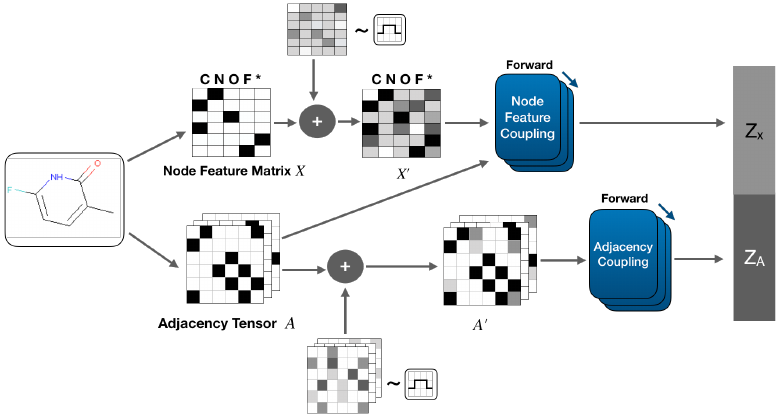
\includegraphics[width=10cm]{graphNVP_Figure1.png}
\caption{For the forward transform, A and X matrices are perturbed by uniform noise. The node coupling is conditioned on the A matrix.}
\end{figure}

\begin{figure}[ht]
\centering
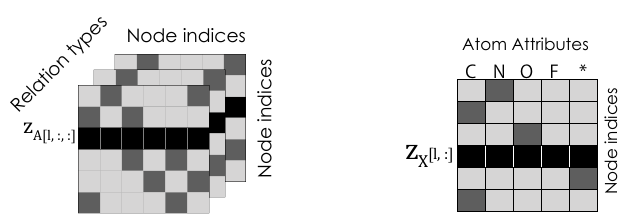
\includegraphics[width=6cm]{graphNVP_Figure2.png}
\caption{The coupling structure splits the A and X matrices as one node vs all the rest. This works best in experiments, though breaks down permutation invariance.}
\end{figure}

\begin{figure}[ht]
\centering
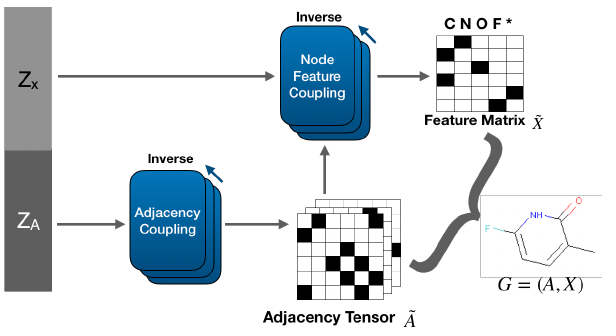
\includegraphics[width=8cm]{graphNVP_Figure3.png}
\caption{Generation is in two steps because the reverse coupling transform of X is conditioned on A so this needs to be generated first. Using simple dequantization (flooring) to get from continuous flow output to discrete A, X.}
\end{figure}

\textbf{Experiments:} on QM9\index{QM9} and ZINC-250K\index{ZINC} with kekulized graphs (without hydrogens) - our \emph{cheat} version.
Have not so great validity but high uniqueness.
Claim benefits in speed of generation as opposed models that have complex decoders checking the validity of molecules in the process.
Some comments on smoothness of latent space and possibility to interpolate for property control but not very convincing.


\clearpage

\section{MPGVAE}\label{sec:MPGVAE}\index{MPGVAE}

\begin{notebox}
\textbf{Paper: } \fullcite{flam-shepherd_mpgvae_2021}
\vspace{5pt}

no reviews
\hspace{1cm}
no official code
\hspace{1cm}
\href{Flam-Shepherd et al_2021_MPGVAE.pdf}{Local pdf}

\hfill Notes taken: 6/2/2022 \index{February 2022}
\end{notebox}

\begin{notebox}[colback=red!5]
\tldr Federated learning setup where server has data with labels and clients have unlabelled data, moreover with some 
\end{notebox}

\begin{notebox}[colback=yellow!5]
\textbf{Notes:} 
\begin{itemize}[nosep]
\item presented by Manual at CAIRO readings 6/2/2022
\end{itemize}
\end{notebox}


Graph with adjacency matrix, edge feature tensor and node feature matrix $G = (A, E, X)$.
Assume independence between node and edge probability distributions (Erdos-R\'enyi graph model) such as in \citetitle{simonovsky_graphvae_2018} of \textcite{simonovsky_graphvae_2018}\index{GraphVAE}.

Starting point is standard VAE and ELBO. Both edge and node features are categorical.
Build a message passing NN (MPNN)\index{message passing NN} into encoder and decoder of the VAE.

Refers to Graphite from Grover et al 2018 as nearest baseline - how different is this?

\begin{figure}[ht]
\centering
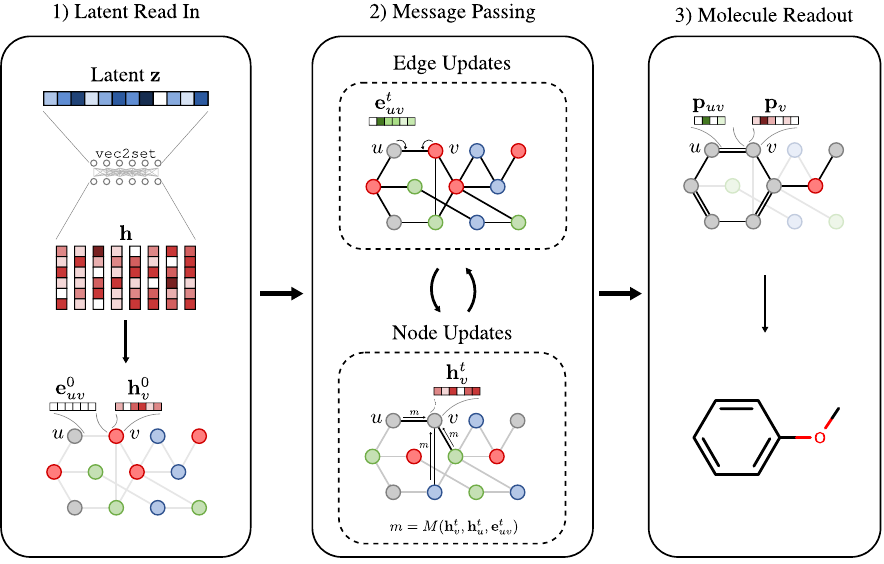
\includegraphics[width=10cm]{mpgvae_figure1.png}
\caption{1) Read in latent $z$ by passing it through linear layer to get to correct node dimensions and pass it through RNN to get initial node featues. Edge features fixed to zero - unconnected graph. 2) Message passing on both, node and edge representations. 3) Use last node and edge representation to predict independent node and edge feature probabilities.}
\end{figure}

Claim that has lower complexity than GrpahVAE (how so?).

\textbf{Encoder:} Use MPNN to map node and edge representations into latent space.
Messages are constructed at edge level as linear functions of itself, neighbouring nodes, and edge features passed through tanh nonlinearity.
Edge updates are directly the messages. 
Node updates first use attention to reweight the messages and then pass it through a GRUCell (this is not very clear, there is something strange in eq. 11 - should be a message for u only? not uv?)
Use set2set from Vinyals 2015 (unlike in seq2seq, in sets the order should not matter and the model should produce the same representation in arbitrary ordering of the set) to read from last node representation to fixed-sized hidden representation $z$.

\textbf{Decoder:} Pass latent through linear layer to expand dims and then RNN to get initial node featurs (edge features zero - unconnected graph). MPNN identical to encoder - update both nodes and eges.
Readout the last layer into stochastic graph representation by passing it through single layer NN and softmax.

\textbf{Experiments:} Over QM9 (not clear whether kekulized or not and if has hydrogens) - best validity compared to GrphVAE, MolGAN, CharacterVAE and Grammar VAE. Generate $10^4$ molecules and achieve validity over 90\%, unique almost 70\% and novel about 50\% - much better then baseline. 
Also evaluates the continuous (chemical properties) and discrete (avg number of atom types and ring size) property distributions of generated vs training sample graphs - claim to have both better than baseline.





\clearpage

\section{FMTDA}\label{sec:FMTDA}\index{FMTDA}

\begin{notebox}
\textbf{Paper: } \fullcite{yao_federated_2022}
\vspace{5pt}

\href{https://openaccess.thecvf.com/content/WACV2022/html/Yao_Federated_Multi-Target_Domain_Adaptation_WACV_2022_paper.html}{reviews not available}
\hspace{1cm}
{No code}
\hspace{1cm}
\href{run:/home/magda/Dropbox/Zot/Yao et al_2022_Federated multi-target domain adaptation.pdf}{Local pdf}
\vspace{3pt}

Presented by Manuel\index{Manuel} in CAIRO readings on 9/2/2022
\hfill Notes taken: 13/2/2022 \index{February 2022}
\end{notebox}

\begin{notebox}[colback=red!5]
\tldr Federated learning\index{federated learning} (FL) setup where server has labelled data and clients have only unlabelled data moreover with shifted data domains. Builds on maximum classifier discrepancy (MCD) [39] training which is a kind of adversarial game with minimax loss where there are two classifiers acting as discriminators and a feature extractor acting as a generator. The generator tries to align the features between the source and target domains and the discriminator step uses two classifiers that try to disagree as much as possible on the target domain while being correct for the source domain. 
In the FL setup they discuss here the problem is all about what is trained where and how it is communicated. Feature extractor needs to be trained on the server together with a global classifier while local classifiers are trained on the clients. The data domains are modelled by a simple GMM which is used to re-weight examples when calculating the classification losses for within and out of distribution data examples.
\end{notebox}

\begin{notebox}[colback=yellow!5]
\textbf{Notes:} 
\begin{itemize}[nosep]
\item Nice paper as not so trivial intro to FL
\item Experiments still surprisingly low accuracy - 30\% on MNIST like data.
\item Possible future work\index{future work}: take on board new clients with new target domains quickly (cannot retrain the whole system every time there is a new client). Use GMMs to find the nearest domain and initialize new client by this classifier. Adapt only client and server and gradually spread?\index{idea}
\end{itemize}
\end{notebox}

\begin{wrapfigure}{r}{0.5\textwidth}
\centering
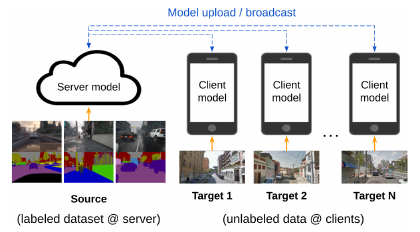
\includegraphics[width=0.5\textwidth]{fmtda_Figure1.png}
% \caption{Federated learning (FL) setup in which the server has labelled data and the clients have unlabelled data. Moreover, the data domains on the server (source domain $D_S$) and the clients (target domains $D_T$) are assumed to be not (perfectly) aligned.}
\end{wrapfigure}
Federated learning (FL) setup in which the server has labelled data and the clients have unlabelled data. Moreover, the data domains on the server (source domain $D_S$) and the clients (target domains $D_T$) are assumed to be not (perfectly) aligned.

Model aggregation on the server in this case won't work because of inter-client discrepancies. Instead they propose dual adaptation approach whereby the models are adapted both at the server and the clients. The models are based on a common feature extractor $G$ and classifier heads $F_i$.

They reuse the maximum classifier discrepancy (MCD) approach introduced in [34 ref in the paper] which has similar minimax game as GAN.
\begin{figure}[ht]
\centering
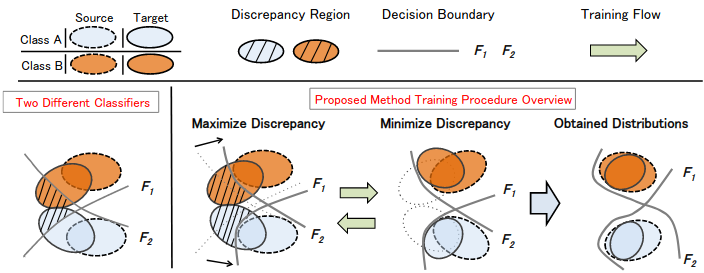
\includegraphics[width=10cm]{fmtda_Figure3.png}
\caption{34 MCD: On one hand train 2 classifiers $F_1$ and $F_2$ that perform well on the source domain but at the same time maximize the classification discrepancy (discriminators) in the target domain. On the other train the feature extractor (generator) to fool the discriminators, that is minimize the discrpancy. This shall push the target features into the source domain.}
\end{figure}
\begin{align*}
\text{Discriminator loss: } \quad & \argmin_{F_1, F_2} \Ls_{ce}(D_S) - \Ls_{adv}(D_T) \\
\text{Generator loss: } \quad & \argmin_{G} \Ls_{adv}(D_T) \enspace , 
\end{align*}
where $\Ls_{ce}(D_S)$ is standard cross-entropy loss over the labelled source domain and is a suitable discrepancy loss such as $L^1$ norm that they use here $\Ls_{adv}(D_T) \E_{\rvx \sim D_T} \Vert F_1(G(\rvx)) - F_2(G(\rvx)) \Vert_1$.
\begin{wrapfigure}{l}{0.5\textwidth}
\centering
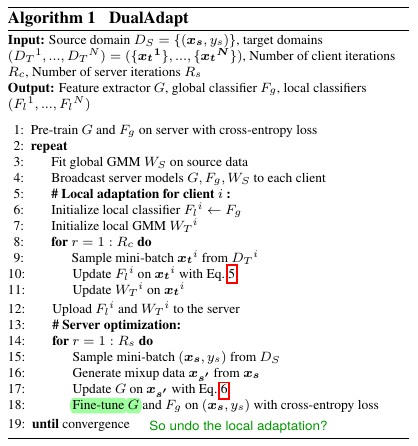
\includegraphics[width=0.5\textwidth]{fmtda_Algo.png}
\end{wrapfigure}

In their setup they update the generator (feature extractor) $G$ on the server and have a global classifier $F_g$ on the server and local classifiers $F_t^i$ on the clients.
They train the local classifiers $f_t^i$ via the discriminator loss by maximizing the $\Ls_{adv}$ discrepancy between the global (fixed here) and local classifiers together with minimizing the cross-entropy using the predictions of the global classifier $F_g$ as the ground truth.
Since the labels from $F_g$ may not be perfect, they use GMM fitted on $D_S$ to re-weight the target examples (if out of source distribution, should have lower weight).

They also fit GMM on the clients. These local GMMs are uploaded together with the local classifiers to the server. The feature extractor $G$ is trained on the server by minimizing the generator loss with $\Ls_{acv}$ evaluated over mix-up instances (simple avg of two randomly sampled instances from $D_S$) weighted by local GMM mixtures. This is done for each target domain so that the server loss is the average across all the target models.

\begin{figure}[ht]
\centering
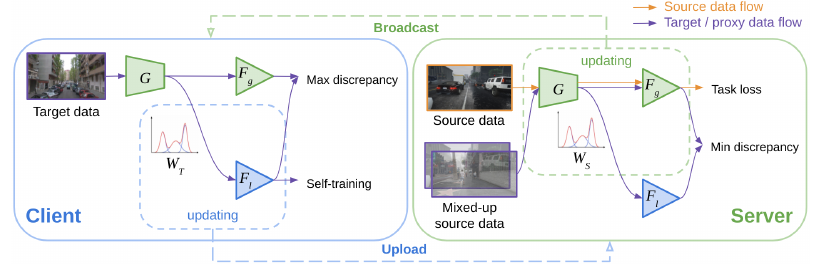
\includegraphics[width=12cm]{fmtda_Figure2.png}
\caption{Dual model adaptation on both clients and server.}
\end{figure}

At inference they classify new instances by averaging the global and local classifier predictions. 

They show experiments on MNIST as the source domain and MNIST-M, SVHN, USPS etc. as targets; DomainNet (clipart, infograph, painting .. )and GTA5 dataset with street-views simulated from computer games. It seems to perform better then baselines though still only about 30\% accuracy on MNIST-like data.



\clearpage

\section{Diffusion models}\label{sec:Diffusion}\index{denoising diffusion}\index{diffusion model}

\begin{notebox}
\textbf{Paper: } \fullcite{ho_denoising_2020}
\vspace{5pt}

\href{https://proceedings.neurips.cc/paper/2020/hash/4c5bcfec8584af0d967f1ab10179ca4b-Abstract.html}{reviews}
\hspace{1cm}
\href{https://github.com/hojonathanho/diffusion}{code}
\hspace{1cm}
\href{run:/home/magda/Dropbox/Zot/Ho et al_2020_Denoising Diffusion Probabilistic Models.pdf}{Local pdf}
\vspace{3pt}

Read with Simon on 27/1/2022
\hfill Notes taken: 13/2/2022 \index{February 2022}
\end{notebox}

\begin{notebox}[colback=red!5]
\tldr Diffusion process is a Markov chain gradually adding small quantities of noise to the data until the signal is completely destroyed - seems as random noise. 
The diffusion model is trained to reverse this process.
When the diffusion consists of Gaussian noise, the sampling transitions can be Gaussian as well.
The diffusion (forward) process is seen as a posterior $q(\rvx_{t} \vert \rvx_{t-1})$ of the reverse model $p_{\theta}(\rvx_{t-1} \vert \rvx_{t})$.
Here, however, the posterior is fixed (Gussians with variance schedule) so that the full chain $\rvx_{1:T}$ can be generated from the data $\rvx_0$ and the model is then trained to get back using variational lower bound on $\log p_{\theta}(\rvx_0)$ as the loss. The trick is in rewriting the lower bound so that it is trainable. It all relies on tractability of the conditionals because they are all Gaussians.
\end{notebox}

\begin{notebox}[colback=yellow!5]
\textbf{Notes:} 
\begin{itemize}[nosep]
\item What if the Markov chain was not Gaussian? Would it still be possible to find a tractable solution and would it be good for anything?\index{idea} Probably not. The initial generative noise would then be non-Gaussian - so what?
\end{itemize}
\end{notebox}


\begin{figure}[ht]
\centering
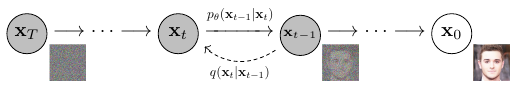
\includegraphics[width=12cm]{diffusion_Figure1.png}
\caption{Forward diffusion process $q$ and reverse diffusion model $p$.}
\end{figure}
Diffusion model is latent variable model 
$p_{\theta}(\rvx_0) = \int p_{\theta}(\rvx_{0:T}) d\rvx_{1:T}$ where the latents $\rvx_{1:T}$ have the same dims as the data $\rvx_0 \sim q(\rvx_0)$.
The joint distribution called the \emph{reverse process}\index{reverse process} is a Markov chain with learned Gaussian transitions
\begin{align*}
p_{\theta}(\rvx_{0:T}) = p(\rvx_T) \Pi_{t=1}^T p_{\theta}(\rvx_{t-1} \vert \rvx_{t}), \qquad p_{\theta}(\rvx_{t-1} \vert \rvx_{t}) = \mathcal{N}(\rvx_{t-1}; \mu_{\theta}(\rvx_t, t), \Sigma_{\theta}(\rvx_t, t))
\end{align*}

The diffusion process (\emph{forward process}\index{forward process}) is also a Markov chain adding gradually Gaussian noise to the data and is the approximate posterior of the model
\begin{align*}
q(\rvx_{1:T} \vert \rvx_0) = \Pi_{t=1}^T q(\rvx_{t} \vert \rvx_{t-1}), \qquad q(\rvx_{t} \vert \rvx_{t-1}) = \mathcal{N}(\rvx_{t}; \sqrt{1 - \beta_t}\rvx_{t-1}, \beta_t \mI) \enspace , 
\end{align*}
where $\beta_1, \ldots, \beta_T$ is a variance schedule.

Training is done by maximizing the usual variational lower bound on $\log p_{\theta}(\rvx_0)$ with the whole $\rvx_{1:T}$ as latent and using the Markov chain properties to decompose it into a sum of KL divergences over the chain conditionals $q(\rvx_{t} \vert \rvx_{t-1})$.
$\beta$'s can be trained by reparametrization trick or fixed as hyperparameters.

Interestingly, due to the specific formulation of the forward process, any timestep $t$ can be sampled using only the initial point $\rvx_0$ for conditioning 
\begin{align*}
q(\rvx_{t} \vert \rvx_0) = \mathcal{N}(\rvx_{t}; \sqrt{\bar\alpha_t}\rvx_{0}, 1-\bar\alpha_t \mI), \qquad \alpha_t = 1 - \beta_t, \ \bar\alpha_t = \Pi_{s=1}^t \alpha_s
\end{align*}
Due to this, the forward process Markov chain conditionals (the posteriors) are tractable when conditioned on $\rvx_0$
\begin{align*}
q(\rvx_{t} \vert \rvx_{t-1}, \rvx_0) = \mathcal{N}(\rvx_{t}; \bar\mu(\rvx_t, \rvx_0), \bar\beta_t \mI) \enspace ,
\end{align*}
where $\bar\mu$ is a fixed simple function of $\rvx_t, \rvx_0$ and some $\alpha$s and $\beta$s (see equation 7 in paper for details).

In their setup they do not learn $\beta$s but fix them - approximate posterior has no trainable parameters (no $\theta$s in the above), forward process is fixed.

The reverse process $p_{\theta}(\rvx_{t-1} \vert \rvx_{t}) = \mathcal{N}(\rvx_{t-1}; \mu_{\theta}(\rvx_t, t), \Sigma_{\theta}(\rvx_t, t))$ has in principal trainable mean and variance functions but they fix the variance to isotropic $\sigma_t \mI$ ($\sigma_t$ is a simple fixed function of $\beta_t$ - see paper).
With these the KL divergences in the ELBO loss can be evaluated in closed form (boil down to $\ell_2$ norms) and the only thing we learn are the mean functions $\mu_{\theta}(\rvx_t, t)$ of the $t-1$ step in the reverse process.

We can further reparametrize the sampling of $x_t$ by sampling the standard normal $\epsilon \sim \mathcal{N}(0, \mI)$ and $x_t = \sqrt{\bar\alpha_t}\rvx_{0} + \sqrt{1-\bar\alpha_t} \epsilon$ and hence $\rvx_0 = (\rvx_t - \sqrt{1-\bar\alpha_t} \epsilon) / \sqrt{\bar\alpha_t}$.
This does not seem very useful cause we do not learn any of the parameters. 
However, since by the loss the mean of the reverse process at step $t$ shall be the same as the mean of the forward process (which is obtainable in closed from from $\alpha$s and $\beta$s and the actual values of $\rvx$ generated by the forward process), we get that 
\begin{align*}
\mu_{\theta}(\rvx_t, t) = \frac{1}{\sqrt{\bar\alpha_t}}(\rvx_t - \sqrt{1-\bar\alpha_t} \, \epsilon_\theta(\rvx_t, t)) \enspace ,
\end{align*}
where $\epsilon_\theta(\rvx_t, t)$ is the function that shall be trained to minimize the ELBO.
To sample, we use $\rvx_{t-1} = \frac{1}{\sqrt{\bar\alpha_t}}(\rvx_t - \sqrt{1-\bar\alpha_t} \, \epsilon_\theta(\rvx_t, t)) + \sigma_t \rvz, \ \rvz \sim \mathcal{N}(0, \mI)$ recursively starting from $\rvx_t \sim \mathcal{N}(0, \mI)$ all the way back to $\rvx_0$.

With the introduction of $\epsilon$ the loss now resembles denoising score matching of \cite{song_generative_2020} and the sampling process the Langevin dynamics.

Nice experiments.














\clearpage

\section{Score-based models}\label{sec:scorebased}\index{score-based models}

\begin{notebox}
\textbf{Paper: } \fullcite{song_generative_2020}
\vspace{5pt}

\href{https://papers.nips.cc/paper/2019/file/3001ef257407d5a371a96dcd947c7d93-Reviews.html}{reviews}
\hspace{1cm}
\href{https://github.com/yang-song/score_sde_pytorch}{code}
\hspace{1cm}
\href{run:/home/magda/Dropbox/Zot/Song_Ermon_2020_Generative Modeling by Estimating Gradients of the Data Distribution.pdf}{Local pdf}
\vspace{3pt}

Read with Simon\index{Simon} on 9/2/2022
\hfill Notes taken: 14/2/2022 \index{February 2022}
\end{notebox}

\begin{notebox}[colback=red!5]
\tldr 
\end{notebox}

\begin{notebox}[colback=yellow!5]
\textbf{Notes:} 
\begin{itemize}[nosep]
\item 
\end{itemize}
\end{notebox}


Generative model where data are generated through Langevin dynamics \parencite{welling_bayesian_nodate} using gradients estimated through score matching \parencite{hyvarinen_estimation_nodate}.

They perturb the data with small Gaussian noise to ensure the data don't lie on a low dimensional manifold within the original feature space which would make the gradients ill-defined. They also propose to anneal the Langevin dynamics sampling process with gradually decreasing noise levels.

The model is based on estimating the (Stein) score\index{index} that is the gradient of the log data density with respect to the data $\nabla_{\rvx} \log p(\rvx)$ (though standard score function in statistics is the gradient with respect to the parameters of the distribution at a fixed data point - this is acknowledged in the original [33] paper of Jordan's group but not in this paper).

The score network $s_\theta: R^D \to R^D$ shall be trained to estimate the score without estimating the data likelihood $p(\rvx)$ first. Once trained, it can be used within Langevin dynamics sampling to generate new data examples.

The score matching objective is the minimization of $0.5 \E_{p_{data}} \Vert s_{\theta}(\rvx) - \nabla_{\rvx} \log p(\rvx) \Vert_2^2$ which has been show (in \cite{hyvarinen_estimation_nodate} to be equivalent to the minimization of
\begin{align*}
\E_{p_{data}}(\rvx) \left[ tr(\nabla_\rvx s_\theta(\rvx)) + \frac{1}{2} \Vert s_\theta(\rvx) \Vert_2^2 \right]
\end{align*}

They use score matching from \parencite{hyvarinen_estimation_nodate}


\clearpage

\section{STARTUP}\label{sec:startup}\index{STURTUP}

\begin{notebox}
\textbf{Paper: } \fullcite{phoo_self-training_2021}
\vspace{5pt}

\href{https://openreview.net/forum?id=O3Y56aqpChA}{reviews}
\hspace{1cm}
\href{https://github.com/cpphoo/STARTUP}{code}
\hspace{1cm}
\href{run:/home/magda/Dropbox/Zot/Phoo_Hariharan_2021_Self-training for Few-shot Transfer Across Extreme Task Differences}{Local pdf}
\vspace{3pt}

Presented at CAIRO readings\index{CAIRO readings} 16/2/2022
\hfill Notes taken: 15/2/2022 \index{February 2022}
\end{notebox}

\begin{notebox}[colback=red!5]
\tldr Few-shot learning\index{few-shot learning} when the source domain is very different from the target domain. Solution is in self-training - the teacher on the source domain and student on unlabelled dataset from the target domain labelled using the teacher, combined with self-supervised training (simCLR) over the unlabelled target domain to extract sensible features. They claim that the distances (similarities) induced by the teacher trained over the base domain may be useful even though the classes are different.
\end{notebox}

\begin{notebox}[colback=yellow!5]
\textbf{Notes:} 
\begin{itemize}[nosep]
\item Mixing the best of self-supervised training (simCLR) with teacher-student to transfer from base to target. Seems rather obvious in retrospect but one has to know all these first :)
\item They claim that the groupings (similarities/ distances) induced by the teacher trained over the base domain may be useful in the target domain. This hints towards similarity in the datasets. If these are useful (sensible), it means the base and target datasets are somehow similar. If they are completely different, these won't make sense anyway.
\end{itemize}
\end{notebox}

In cross-domain setups current sota few-shot methods are often outperformed by simple transfer of features from the based domain with finetunning on the target domain \parencite{wallace_extending_2020,guo_broader_2020}.

Here they assume that in addition to the few-shot training set in the target domain they also have a somewhat larger unlabelled dataset that they can use for self-training\index{self-training}.
Since this is not big enough, they, however, still want to use the base dataset to train a teacher\index{teacher-student model}\index{student-teacher model} feature extractor that will be finetuned by a student in the target domain using the teacher to create fake labels. 

\begin{figure}[ht]
\centering
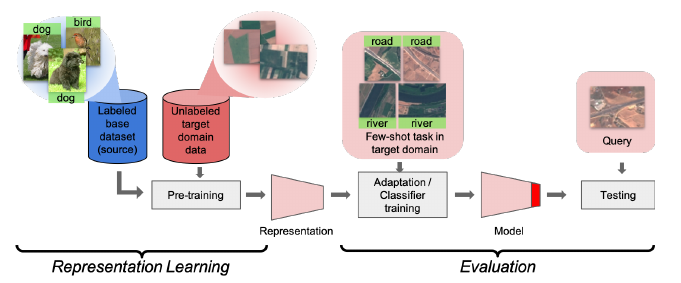
\includegraphics[width=10cm]{startup_Figure1.png}
\caption{Learn representation with self-training and self-supervised training and use for few-shot classification.}
\end{figure}

They claim this can work since the teacher trained over the base (source) domain when used as classifier over the target domain induces \emph{groupings} corresponding to some notion of \emph{similarity and distance} and that the student trained over the target domain with fake labels from the teacher tries to replicate these while adapting to the new domain.

The classification model is $f_{\theta} = C \circ \phi$, where $\phi$ is the feature extractor and $C$ is the classifier with outputs $p(y|x)$. STARTUP does the following
\begin{enumerate}[nosep]
\item Train teacher model $\theta_0$ over base datset $\mathcal{D}_B$
\item Use teacher model to label unlabelled target data $\bar{y}_i = f_{\theta_0}(\rvx_i), \ \rvx_i \in \mathcal{D}_u$
\item Learn student model $\theta^*$ on base and unlabelled target domain
\begin{align*}
\theta^* = \argmin_\theta \frac{1}{N_B} \sum_{(\rvx_i, y_i) \in \mathcal{D}_B} l_{CE}(f_\theta(\rvx_i), y_i) + \frac{1}{N_u} \sum_{(\rvx_i) \in \mathcal{D}_u} KL(f_\theta(\rvx_i), f_{\theta_0}(\rvx_i)) + l_{ss}(\mathcal{D}_u) \enspace ,
\end{align*}
where $l_{CE}$ is a standard cross-entropy loss, $l_{ss}$ is self supervised simCLR loss \parencite{chen_simple_2020}.
\item Train linear classifier on target domain with features $f_{\theta^*}(\rvx)$.
\end{enumerate}

\begin{notebox}
They use KL instead of a simple cross-entropy over the fake labels in the target domain. They don't really comment on this rather then some not very solid argumentation about this emphasizing the groupings induced by the teacher. For me, it has mainly a regularization effect to reduce the trust of the student in the labels produced by the teacher - which is more similar to the original arguments of \cite{xie_self-training_2020} for the need of adding noise into the student not to overfit the teacher
\begin{align*}
KL(f_\theta(\rvx), f_{\theta_0}(\rvx)) = \sum_c f^{c}_\theta(\rvx) \log \frac{f^{c}_\theta(\rvx)}{f^{c}_{\theta_0}(\rvx)} = - \sum_c f^{c}_\theta(\rvx) \log f^{c}_{\theta_0}(\rvx) + \sum_c f^{c}_\theta(\rvx) \log f^{c}_\theta(\rvx) \enspace ,
\end{align*}
which is the minimization of cross-entropy and the maximization of the entropy of $f_\theta$, hence the regularization effect.
\end{notebox}

They discuss a bit the role of the teacher in the initialization of the student and self-supervised feature extractor and the final classifier and go for a reasonable compromise of not using it for the classifier. 

The experiments use miniImigeNet\index{miniImageNet} as the base dataset (60k 84x84 images in 100 classes) and the target domains are Chest x-rays, CropDisease (leafs of plants), EuroSAT (satellite land use), ISIC (melanoma from skin lesions). It beats baselines on all but ChestX and ISIC very difficult (20\%-30\% accuracy for 1-shot 5-way classification). 


\clearpage

\section{MLP-Mixer}\label{sec:mlpmixer}\index{MLP-Mixer}

\begin{notebox}
\textbf{Paper: } \fullcite{phoo_self-training_2021}
\vspace{5pt}

\href{https://openreview.net/forum?id=EI2KOXKdnP}{reviews}
\hspace{1cm}
\href{https://github.com/lucidrains/mlp-mixer-pytorch}{code}
\hspace{1cm}
\href{run:/home/magda/Dropbox/Zot/Tolstikhin et al_2021_MLP-Mixer.pdf}{Local pdf}
\vspace{3pt}

Read with Simon\index{Simon} 24/2/2022
\hfill Notes taken: 1/3/2022 \index{March 2022}
\end{notebox}

\begin{notebox}[colback=red!5]
\tldr CNNs and attention-based models (vision transformers) are state of the art in high-dimensional computer vision problems but they are not necessary. MLP architecture with spatial and channel mixing uses standard MLP operations over data with transposed layout and can achieve similar results with at competitive training times and inference throughput capacity. So not beating anybody but showing that complex architectures are not necessary.
\end{notebox}

\begin{notebox}[colback=yellow!5]
\textbf{Notes:} 
\begin{itemize}[nosep]
\item Why exploring accuracy on downstream task with pre-training on ImageNet and ImageNet21-K and not directly on the ImageNet data? Would it not show so good results?
\item They claim CNN bring into the modeling inductive biases which they do not need. But their patch and channel based architecture and operations are also inductive biases. For normal tabular data or for sequences, these would have to be different.
\end{itemize}
\end{notebox}

CNNs and attention-based models (vision transformers) are state of the art in high-dimensional computer vision problems. Here they propose \iterm{MLP-mixer} which relies on standard MLP architecture with changes to data layout (reshapes and transpose).
It separates the per-location \iterm{channel mixing} and cross-location \iterm{token-mixing} operations (both simple MLPs with parameter sharing) and applies one after the other to each patch representation across the channels and then to each channel across the patch representations (the latter is simply applied to transposed data). The representation dimensions are preserved through these operations (though the inner MLP dimension can be different) so that there can be skip connections.

Most of the paper is about experiments - accuracy on downstream tasks with pre-training on ImageNet and ImageNet21-K.
MLP-Mixer has comparable accuracy to sota CNN and transformer models and at the same time high throughput at inference time and competitive training time.
Unlike CNN-based methods it is also resistant to within-patch pixel permutations and somewhat better adapted to full image permutations.
The extracted features at higher layers are simpler shapes with opposite phases, at deeper layers they have not apparent structure.

\begin{figure}[ht]
\centering
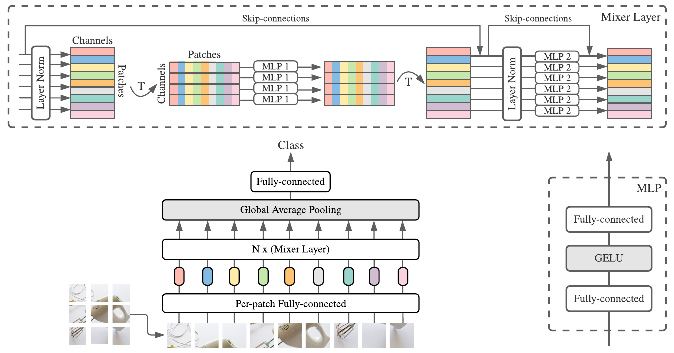
\includegraphics[width=0.9\textwidth]{mlpmixer_Figure1.png}
\caption{MLP-mixer: First all patches are linearly projected with the same projection matrix. Then multiple Mixer Layers are applied and with final global average pooling and fully connected layer for the classification.}
\end{figure}




\clearpage 
\printbibliography



% print index
\phantomsection
\cleardoublepage
\addcontentsline{toc}{section}{\indexname}
\printindex

\end{document}
